\begin{exercise}{Foudre dans un pré}{2}{Spé}
{Electrostatique}{correge}

Un éclair frappe le sol au milieu d'un pré, à proximité d'une vache. Nous cherchons à savoir si cette vache est en sécurité. On modélise la foudre par un fil rectiligne vertical semi-infini, parcouru par un courant $I$. La vache se trouve à une distance $d$ du point d'impact, et la distance entre ses pattes est notée $p$. 

\begin{center}
    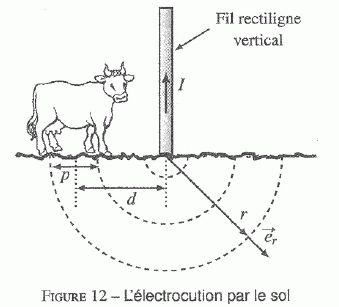
\includegraphics[width=0.4\linewidth]{electromag/electrostat/vache_foudre.png}
\end{center}

\begin{questions}

    \question Déterminer la densité de courant électrique $\vec{j}$ dans le sol.
    \question Rappeler l'expression de la loi d'ohm locale. Exprimer le champ électrique dans le sol et en déduire son potentiel $V(r)$ en le supposant nul à l'infini.
    \question Exprimer en fonction de $p$ et $d$ les potentiels au niveau des pattes avant et arrière de la vache. Quelle est la tension entre les pattes de la vache ?
    \question A quelle distance minimale $d_m$ du point d'impact est-elle en sécurité ?
    
    
    
\end{questions}

\paragraph{Données :} 
\begin{itemize}
    \item Foudre : $I=\SI{15}{kA}$
    \item Conductivité électrique du sol : $\gamma = \SI{1}{S/m}$
    \item Résistance de la vache : $R= \SI{30}{k\Omega}$
    \item Distance entre les pattes : $p=\SI{1.5}{m}$
    \item Courant létal pour une vache : $I_{max} = \SI{25}{mA}$
\end{itemize}

\end{exercise}

\begin{solution}
\begin{questions}

    \question $\vec j(r) = \frac{-I}{2\pi r^2} \vec{e}_r$
    \question $V(r) = \frac{-I}{2\pi \gamma  r} $
    \question $U = V(d+\frac{p}{2}) - V(d+\frac{p}{2}) \approx \frac{Ip}{2\pi \gamma d^2} $
    \question $d_m = \sqrt{\frac{Ip}{2\pi \gamma R I_{max} }}$
    
\end{questions}
\end{solution}
